\chapter{Formal analysis using Alloy}
		\section{World model}
			\lstinputlisting[language=alloy]{alloy/Alloy.als}
		\section{Generated world}
			\subsection{Generic world}
				\paragraph{}
					This is an example of a generic world
					\begin{figure}[!h]
						\includegraphics[width=\textwidth]{images/Alloy/GenericWorld.png}
						\caption{Alloy generic world}
					\end{figure}
			\subsubsection{Municipal wolrd}
				\paragraph{}
					This world highlights the associations occurring into a municipality, such as received reports, issued tickets, occurred accidents and suggested improvements. It also shows how positions are related to municipalities and what occurred on them.
					\begin{figure}[!h]
						\includegraphics[width=\textwidth]{images/Alloy/MunicipalWorld.png}
						\caption{Alloy municipal world}
					\end{figure}
			\subsubsection{User world}
				\paragraph{}
					This world highlights the associations between users and reports.
					\begin{figure}[!h]
						\includegraphics[width=\textwidth]{images/Alloy/UserWorld.png}
						\caption{Alloy user world}
					\end{figure}
			\subsubsection{Add report}
				\paragraph{}
					It shows how a "add report" event occurred
					\begin{figure}[!h]
						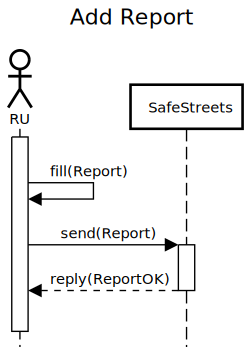
\includegraphics[width=\textwidth]{images/Alloy/AddReport.png}
						\caption{Alloy add report}
					\end{figure}
	